\documentclass[11pt]{book}

\usepackage{amsmath}
\usepackage{amssymb}
\usepackage{amsthm}
\usepackage{mathtools}

\newtheoremstyle{example} % Style name
	{10pt} % Space above
	{10pt} % Space below
	{\normalfont} % Body font
	{} % Header font
	{\bfseries} % Header font
	{.} % Separator
	{10pt} % Space after header
	{} % Header text
\theoremstyle{example}
\newtheorem{example}{Example}[section]
\newtheorem{definition}{Definition}[section]

\begin{document}

\title{Phoenix Dynamics Robotics Manual}
\author{Stewart Nash}

\maketitle

\tableofcontents

\mainmatter

\chapter{Dynamics}

\section{Kinematics}

Take a vector with components $\mathbf{P}=(a_x,b_y,c_z)$. A scale factor $w$ can be added (to the matrix form) to give
\begin{equation}
	\mathbf{P}=
	\begin{bmatrix}
		P_x\\
		P_y\\
		P_z\\
		w
	\end{bmatrix}
\end{equation}
where $(a_x,b_y,c_z)=(P_x/w,P_y/w,P_z/w)$. A direction vector can be represented by a scale factor of zero ($w=0$).

A universe reference frame is represented by $F_{x,y,z}$ and a moving frame is represented by $F_{n,o,a}$ where the letters n, o, and a come from the words normal, orientation and approach. Relative to the gripper, the $z$-axis is the approach axis by which the gripper approaches an object. The orientation with which the gripper frame approaches the part is the orientation axis. The normal-axis or x-axis is normal to both. A fourth vector which gives the location of a frame relative to a reference frame can be added to the vectors representing the components of the $n$-, $o$-, and $a$-axes to give a homogeneous matrix representation of this relative frame
\begin{equation}
	F=
	\begin{bmatrix}
		1&0&0&d_x\\
		0&1&0&d_y\\
		0&0&1&d_z\\
		0&0&0&1
	\end{bmatrix}
\end{equation}
Pre-multiplying the frame matrix by the transformation matrix will yield the new location of the frame.

Rotation matrices about the $x$-, $y$- and $z$-axes are given by
\begin{equation}
	\begin{aligned}
		\mathrm{rot}(x,\theta)&=
		\begin{bmatrix}
			1&0&0\\
			0&\cos{\theta}&\sin{\theta}\\
			0&\sin{\theta}&\cos{\theta}
		\end{bmatrix}\\
		\mathrm{rot}(y,\theta)&=
		\begin{bmatrix}
			\cos{\theta}&0&\sin{\theta}\\
			0&1&0\\
			-\sin{\theta}&0&\cos{\theta}
		\end{bmatrix}\\
		\mathrm{rot}(z,\theta)&=
		\begin{bmatrix}
			\cos{\theta}&-\sin{\theta}&0\\
			\sin{\theta}&\cos{\theta}&0\\
			0&0&1
		\end{bmatrix}
	\end{aligned}
\end{equation}
Denoting the transformation of frame $R$ relative to frame $U$ (universe) as $\prescript{U}{}T_R$, denoting the $p$ relative to the frame $R$ as $\prescript{R}{}p=p_{noa}$, and denoting $p$ relative to frame $U$ as $\prescript{U}{}p=p_{xyz}$ we have
\begin{equation}
	\prescript{U}{}p=\prescript{U}{}T_R\times\prescript{R}{}p
\end{equation}

\subsection{Twists and Screws}

The special orthogonal group is denoted $SO$ and we may define it as the space of rotation matrices in $\mathbb{R}^{n{\times}n}$ by
\begin{equation}
	SO(n)=\{R\in\mathbb{R}^{n{\times}n}:RR^T=I,\mathrm{det}\,R=+1\}
\end{equation}
The space of $n{\times}n$ skew-symmetric matrices is given by
\begin{equation}
	so(n)=\{S\in\mathbb{R}^{n{\times}n}:S^T=-S\}
\end{equation}
The special Euclidean group, generalized to $n$ dimensions, is given by
\begin{equation}
	SE(n)\equiv\mathbb{R}^n\times{SO(n)}
\end{equation}
In other words, the special Euclidean group is comprised of a configuration pair $(p, R)$ which is the product space of $\mathbb{R}^n$ with $SO(n)$ and is given in 3 dimensions by
\begin{equation}
	SE(3)=\{(p,R):p\in\mathbb{R}^3,R\in{SO(3)}\}=\mathbb{R}^3\times{SO(3)}
\end{equation}
We can define $se(n)$ as being comprised of the configuration pair $(v, \omega)$ where $v$ is an element of $\mathbb{R}^n$ and $\omega$ is a skew-symmetric matrix from $so(n)$. In three dimensions we have
\begin{equation}
	se(3)\equiv\{(v,\hat{\omega}):v\in\mathbb{R}^3,\hat{\omega}\in{so(3)}\}
\end{equation}
A \emph{twist} is an element of $se(3)$, $\hat{\xi}\in{se(3)}$. The twist coordinates of $\hat{\xi}$ are given by $\xi\equiv(v,\omega)$.

A rigid body motion which consists of rotation about an axis in space through an angle of $\theta$ radians, followed by a translation along the same axis by and amount $d$ is referred to as a screw motion. A \emph{screw} is composed of an axis $l$, a pitch $h$, and a magnitude $M$.

A generalized force acting on a rigid body consists of a linear component, i.e. a `pure force', and an angular component, i.e. a `pure moment', acting at a point. This generalized force can  be represented as a vector in $\mathbb{R}^6$
\begin{equation}
	F=
	\begin{bmatrix}
		f\\
		\tau
	\end{bmatrix}
\end{equation}
where $f$ is the linear component in $\mathbb{R}^3$ and $\tau$ is the rotational component in $\mathbb{R}^3$. We refer to this force and moment pair as a \emph{wrench}.

\section{Differential Motion}

\section{Dynamic Analysis}

The Lagrangian is given by $L=T-V$ where $T$ and $V$ are the kinetic and potential energy of a system, respectively. If $F_i$ is the summation of all external forces acting on the $i$th generalized coordinate $q_i$, the equations of motion are given by
\begin{equation}
	F_i=\frac{d}{dt}\left(\frac{\partial{L}}{\partial\dot{q}_i}\right)-\frac{\partial{L}}{\partial{q_i}}
\end{equation}
When this is solved, the resulting equations of manipulator dynamics can be written
\begin{equation}
	M(q)\ddot{q}+V(q,\dot{q})+G(q)=\tau
\end{equation}
or, alternatively,
\begin{equation}
	M(q)\ddot{q}+C(q,\dot{q})\dot{q}+N(q,\dot{q})=\tau
\end{equation}
where $M(q)$ is the inertia matrix, $V(q,\dot{q})$ is the Coriolis and centripetal acceleration vector, $C(q,\dot{q})$ is the Coriolis matrix, $G(q)$ is the gravity vector, $N(q,\dot{q})$ represents gravity and other non-linear terms and $\tau$ is the $n$-vector of generalized forces which could be, for example, the actuator torques.

To be concrete, we can give an example of this in which we have two coordinates, $x$ and $\theta$, for the $i$th of $n$ linkages. If $F_i$ is the summation of all external forces for a linear motion and $T_i$ is the summation of all external torques for a rotational motion, then
\begin{equation}
	\begin{aligned}
		F_i&=\frac{d}{dt}\left(\frac{\partial{L}}{\partial\dot{x}_i}\right)-\frac{\partial{L}}{\partial{x_i}}\\
		T_i&=\frac{d}{dt}\left(\frac{\partial{L}}{\partial\dot{\theta}_i}\right)-\frac{\partial{L}}{\partial\theta_i}
	\end{aligned}
\end{equation}
We can simplify the equations of motion for a 2-DOF system which is given by
\begin{equation}
	\begin{bmatrix}
		\tau_i\\
		\tau_j
	\end{bmatrix}=
	\begin{bmatrix}
		M_{ii}&M_{ij}\\
		M_{ji}&M_{jj}
	\end{bmatrix}
	\begin{bmatrix}
		\ddot{\theta}_i\\
		\ddot{\theta}_j
	\end{bmatrix}+
	\begin{bmatrix}
		C_{iii}&C_{ijj}\\
		C_{jii}&C_{jjj}
	\end{bmatrix}
	\begin{bmatrix}
		\dot{\theta}_i\\
		\dot{\theta}_j
	\end{bmatrix}+
	\begin{bmatrix}
		C_{iij}&C_{iji}\\
		C_{jij}&C_{jji}
	\end{bmatrix}
	\begin{bmatrix}
		\dot{\theta}_i\dot{\theta}_j\\
		\dot{\theta}_j\dot{\theta}_i
	\end{bmatrix}+
	\begin{bmatrix}
		G_i\\
		G_j
	\end{bmatrix}
\end{equation}
Where the coefficient $M_{ii}$ is the effective inertia at joint $i$, such that an acceleration at joint $i$ causes a torque at joint $i$ equal to $M_{ii}\ddot{\theta}_i$, and the coefficient $M_{ij}$ is the coupling inertia between joints $i$ and $j$ such that an acceleration at joint $i$ or $j$ causes a torque at joint $j$ or $i$ equal to $M_{ij}\ddot{\theta}_j$ or $M_{ji}\ddot{\theta}_i$. $C_{ijj}\dot{\theta}_j^2$ terms represent centripetal forces acting at joint $i$ due to a velocity at joint $j$. All terms with $\dot{\theta}_i\dot{\theta}_j$ represent Coriolis accelerations and, when multiplied by corresponding inertias, represent Coriolis forces. $G_i$ represents gravity forces at joint $i$.

\section{Trajectory Planning}

\chapter{Controls}

\section{State Variable Representation}

Powerful tools from matrix algebra can be used to solve sets of first-order differential equations. That is why it is sometimes helpful to transform a system described by \emph{n}th-order differential equations into a system of first-order differential equations.

\subsection{Systems Modeled by Linear Differential Equations}

Consider a system represented by a \emph{n}th-order, single-input linear constant coefficient differential equation
\begin{equation}
	\sum_{i=0}^n{a_i\frac{d^iy}{dt^i}}=u
\end{equation}
This equation can be replaced by \emph{n} first-order differential equations
\begin{equation}
	\left\{
		\begin{aligned}
			\frac{dx_k}{dt}&=x_{k+1},\,1<k<n\\
			\frac{dx_n}{dt}&=\frac{1}{a_n}\left[\sum_{k=0}^{n-1}{a_kx_{k+1}}\right]+\frac{1}{a_n}u
		\end{aligned}
	\right.
\end{equation}
where $x_1\equiv{y}$ and $i,k\in\mathbb{W}$. This can be written as a matrix equation
\begin{equation}
	\begin{bmatrix}
		\frac{dx_1}{dt}\\
		\frac{dx_2}{dt}\\
		\vdots\\
		\frac{dx_n}{dt}
	\end{bmatrix}
	\begin{bmatrix}
		0&1&0&\cdots&0\\
		0&0&1&\cdots&0\\
		\vdots&\vdots&\vdots&\ddots&\vdots\\
		-\frac{a_0}{a_n}&-\frac{a_1}{a_n}&-\frac{a_2}{a_n}&\cdots&-\frac{a_{n-1}}{a_n}
	\end{bmatrix}
	\begin{bmatrix}
		x_1\\
		x_2\\
		\vdots\\
		x_n
	\end{bmatrix}+
	\begin{bmatrix}
		0\\
		0\\
		\vdots\\
		0\\
		\frac{1}{a_n}
	\end{bmatrix}u
\end{equation}
or
\begin{equation}
	\frac{d\mathbf{x}}{dt}=A\mathbf{x}+\mathbf{b}u
\end{equation}
A multi-input-multi-output (MIMO) system can be represented by
\begin{equation}
	\begin{bmatrix}
		\frac{dx_1}{dt}\\
		\frac{dx_2}{dt}\\
		\vdots\\
		\frac{dx_n}{dt}
	\end{bmatrix}
	\begin{bmatrix}
		a_{11}&a_{12}&\cdots&a_{1n}\\
		a_{21}&a_{22}&\cdots&a_{2n}\\
		\vdots&\vdots&\ddots&\vdots\\
		a_{n1}&a_{n2}&\cdots&a_{nn}
	\end{bmatrix}
	\begin{bmatrix}
		x_1\\
		x_2\\
		\vdots\\
		x_n
	\end{bmatrix}+
	\begin{bmatrix}
		b_{11}&b_{12}&\cdots&b_{1r}\\
		b_{21}&b_{22}&\cdots&b_{2r}\\
		\vdots&\vdots&\ddots&\vdots\\
		b_{n1}&b_{n2}&\cdots&b_{nr}
	\end{bmatrix}
	\begin{bmatrix}
		u_1\\
		u_2\\
		\vdots\\
		u_r
	\end{bmatrix}
\end{equation}
or
\begin{equation}
	\frac{d\mathbf{x}}{dt}=A\mathbf{x}+B\mathbf{u}\label{eq:3_25}
\end{equation}
where $\mathbf{u}$ is an \emph{r}-vector of input functions.\\
Let $\mathbf{\Phi}$ be the $n\times{n}$ \emph{transition matrix} of the differential equation given above which is described by the matrix equation
\begin{equation}
	\frac{d\mathbf{\Phi}}{dt}=A\mathbf{\Phi}
\end{equation}
If $\mathbf{\Phi}(0)=I$ (initial condition) then $\mathbf{\Phi}(t)=e^{At}$ where
\begin{equation}
	e^{At}=\sum_{n=0}^\infty{\frac{A^nt^n}{n!}}
\end{equation}
The solution to \eqref{eq:3_25} on the interval $0\leq{t}<\infty$ is given by
\begin{equation}
	\mathbf{x}(t)=e^{At}\mathbf{x}(0)+\int_0^t{e^{A(t-\tau)}B\mathbf{u}(\tau)\,d\tau}
\end{equation}

A basic mathematical model for a linear time-invariant system consists of the state differential equation and the algebraic output equation
\begin{align}
	\dot{x}(t)=&Ax(t)+Bu(t)\quad{x(t_0)=x_0}\label{eq:stateeqn}\\
	y(t)=&Cx(t)+Du(t)
\end{align}
As we saw, the closed-form expression for the complete solution, a `variation-of-constants formula' is given by
\begin{equation}
	x(t)=e^{A(t-t_0)}x(t_0)+\int_{t_0}^t{e^{A(t-\tau)}Bu(\tau)\,d\tau}
\end{equation}
The complete output response is given (using substition) by
\begin{equation}
	y(t)=Ce^{A(t-t_0)}x(t_0)+\int_{t_0}^t{Ce^{A(t-\tau)}Bu(\tau)\,d\tau}+Du(t)
\end{equation}
The Laplace transform of the output equation can be taken. In that case, the solution to $X(s)$ is
\begin{equation}
	X(s)=(sI-A)^{-1}x_0+(sI-A)^{-1}BU(s)
\end{equation}
The solution to the output equation is
\begin{align}
	Y(s)&=CX(s)+DU(s)\\
	&=C(sI-A)^{-1}x_0+[C(sI-A)^{-1}B+D]U(s)
\end{align}

\subsection{Controllability}

A state $x\in\mathbb{R}^n$ is controllable to the origin if for a given initial time $t_0$ there exists a finite final time $t_f>t_0$ and a piecewise continuous input signal $u(\cdot)$ defined on $[t_0,t_f]$ such that with inital state $x(t_0)=x_0$, the final state satisfies
\begin{align}
	x(t_f)&=e^{A(t_f-t_0)}x+\int_{t_0}^{t_f}{e^{A(t_f-\tau)}Bu(\tau)\,d\tau}\\
	&=0\in\mathbb{R}^n
\end{align}
The state equation \ref{eq:stateeqn} is controllable if every state $x\in\mathbb{R}^n$ is controllable to the origin.
The controllability matrix is
\begin{equation}
	P=[B\,AB\,A^2B\,\cdots\,A^{n-1}B]
\end{equation}
The linear state equation \ref{eq:stateeqn} is controllable if and only if $\mathrm{rank}\,P=n$.
For any initial time $t_0$ and finite final time $t_f>t_0$, the controllability Gramian is defined as
\begin{equation}
	W(t_0,t_f)=\int_{t_0}^{t^f}{e^{A(t_0-\tau)}BB^Te^{A^T(t_0-\tau)}\,d\tau}
\end{equation}
$\mathrm{rank}\,P=n$ if and only if the controllability Gramian $W(t_0,t_f)$ is nonsingular for any initial and finite final times $t_0<t_f$.

\subsection{Observability}

A state $x_0\in\mathbb{R}^n$ is unobservable if the zero-input response of the linear state equation \ref{eq:stateeqn} with initial state $x(t_0)=x_0$ is $y(t)\equiv{0}$ for all $t\geq{t_0}$. The state equation \ref{eq:stateeqn} is observable if the zero vector $0\in\mathbb{R}^n$ is the only unobservable state.
The observability matrix is
\begin{equation}
	Q=
	\begin{bmatrix}
		C\\
		CA\\
		CA^2\\
		\vdots\\
		CA^{n-1}
	\end{bmatrix}
\end{equation}
The linear state equation \ref{eq:stateeqn} is observable if and only if $\mathrm{rank}\,Q=n$.
For any initial time $t_0$ and finite final time $t_f>t_0$, the observability Gramian is defined as
\begin{equation}
	M(t_0,t_f)=\int_{t_0}^{t^f}{e^{A(\tau-t_0)}C^TCe^{A^T(\tau-t_0)}\,d\tau}
\end{equation}
$\mathrm{rank}\,Q=n$ if and only if the observability Gramian $M(t_0,t_f)$ is nonsingular for any initial and finite final times $t_0<t_f$.

\subsection{Examples}

\begin{example}

Two masses $m_1$ and $m_2$ lie on a frictionless level surface. $m_1$ is to the left of $m_2$. $m_1$ is connected to a wall on the left by a spring and a damper. THe right mass $m_2$ is connected to $m_1$ by a spring and a damper. The with spring which connects $m_1$ to the wall has a spring constant $k_1$ and the damper which connects  $m_1$ to the wall has a damping coefficient of $c_1$. The spring which connects $m_2$ to $m_1$ has a spring constant of $k_2$ and the damper which connects the two masses has a damping coefficient of $c_2$. The displacement of $m_1$ from equilibrium is $y_1(t)$ and the velocity of $m_1$ is $u_1(t)$. The displacement of $m_2$ from equilibrium is $y_2(t)$ and the velocity of $m_2$ is $u_2(t)$. 

We make the following assignments
\begin{align}
	x_1(t)&=y_1(t)&\\
	x_2(t)&=\dot{y}_1(t)&=\dot{x}_1(t)\\
	x_3(t)&=y_2(t)&\\
	x_4(t)&=\dot{y}_2(t)&=\dot{x}_3(t)
\end{align}
This gives us the state-space representation
\begin{align}
	\dot{x}(t)&=Ax(t)+Bu(t)\\
	y(t)&=Cx(t)+Du(t)
\end{align}
where we have
\begin{align}
	A&=
	\begin{bmatrix}
		0&1&0&0\\
		-\frac{k_1+k_2}{m_1}&-\frac{c_1+c_2}{m_1}&\frac{k_2}{m_1}&\frac{c_2}{m_1}\\
		0&0&0&1\\
		\frac{k_2}{m_2}&\frac{c_2}{m_2}&-\frac{k_2}{m_2}&-\frac{c_2}{m_2}
	\end{bmatrix}\\
	B&=
	\begin{bmatrix}
		0&0\\
		\frac{1}{m_1}&0\\
		0&0\\
		0&\frac{1}{m_2}
	\end{bmatrix}\\
	C&=
	\begin{bmatrix}
		1&0&0&0\\
		0&0&1&0
	\end{bmatrix}\\
	D&=
	\begin{bmatrix}
		0&0\\
		0&0
	\end{bmatrix}
\end{align}
\begin{center}
	\begin{tabular}{rrrr}
		\hline
		$i$ & $m_i$ (kg) & $c_i$ (Ns/m) & $k_i$ (N/m)\\
		\hline
		1 & 40 & 20 & 400\\
		2 & 20 & 10 & 200\\
		\hline
	\end{tabular}
\end{center}
We can simulate the open-loop system response with zero initial input and initial state $x_0=[0.1,0,0.2,0]^T$ with the following code:
\begin{verbatim}
import numpy as np
import matplotlib.pyplot as plt
import control

m1 = 40
m2 = 20
k1 = 400
k2 = 200
c1 = 20
c2 = 10

A = np.array([
	[0, 1, 0, 0],
	[-(k1 + k2)/m1, -(c1 + c2)/m1, k2/m1, c2/m1],
	[0, 0, 0, 1],
	[k2/m2, c2/m2, -k2/m2, -c2/m2]
])

B = np.array([
	[0, 0],
	[1/m1, 0],
	[0, 0],
	[0, 1/m2]
])

C = np.array([
	[1, 0, 0, 0],
	[0, 0, 1, 0]
])

D = np.array([
	[0, 0],
	[0, 0]
])

sys = control.StateSpace(A, B, C, D)
T = np.linspace(0, 10, 1000)
U = np.zeros((2, len(T)))
X0 = [0.1, 0, 0.2, 0]
T, y = control.forced_response(sys, T=T, U=U, X0=X0)

plt.figure(figsize=(10, 5))
plt.plot(T, y[0], label="m1 position")
plt.plot(T, y[1], label="m2 position")
plt.title("Zero-input response of example 10-1")
plt.xlabel("Time (s)")
plt.ylabel("Displacement (m)")
plt.grid(True)
plt.legend()
plt.tight_layout()
plt.show()
\end{verbatim}
This gives us the following figure:
\begin{figure}[htbp]
	\centering
	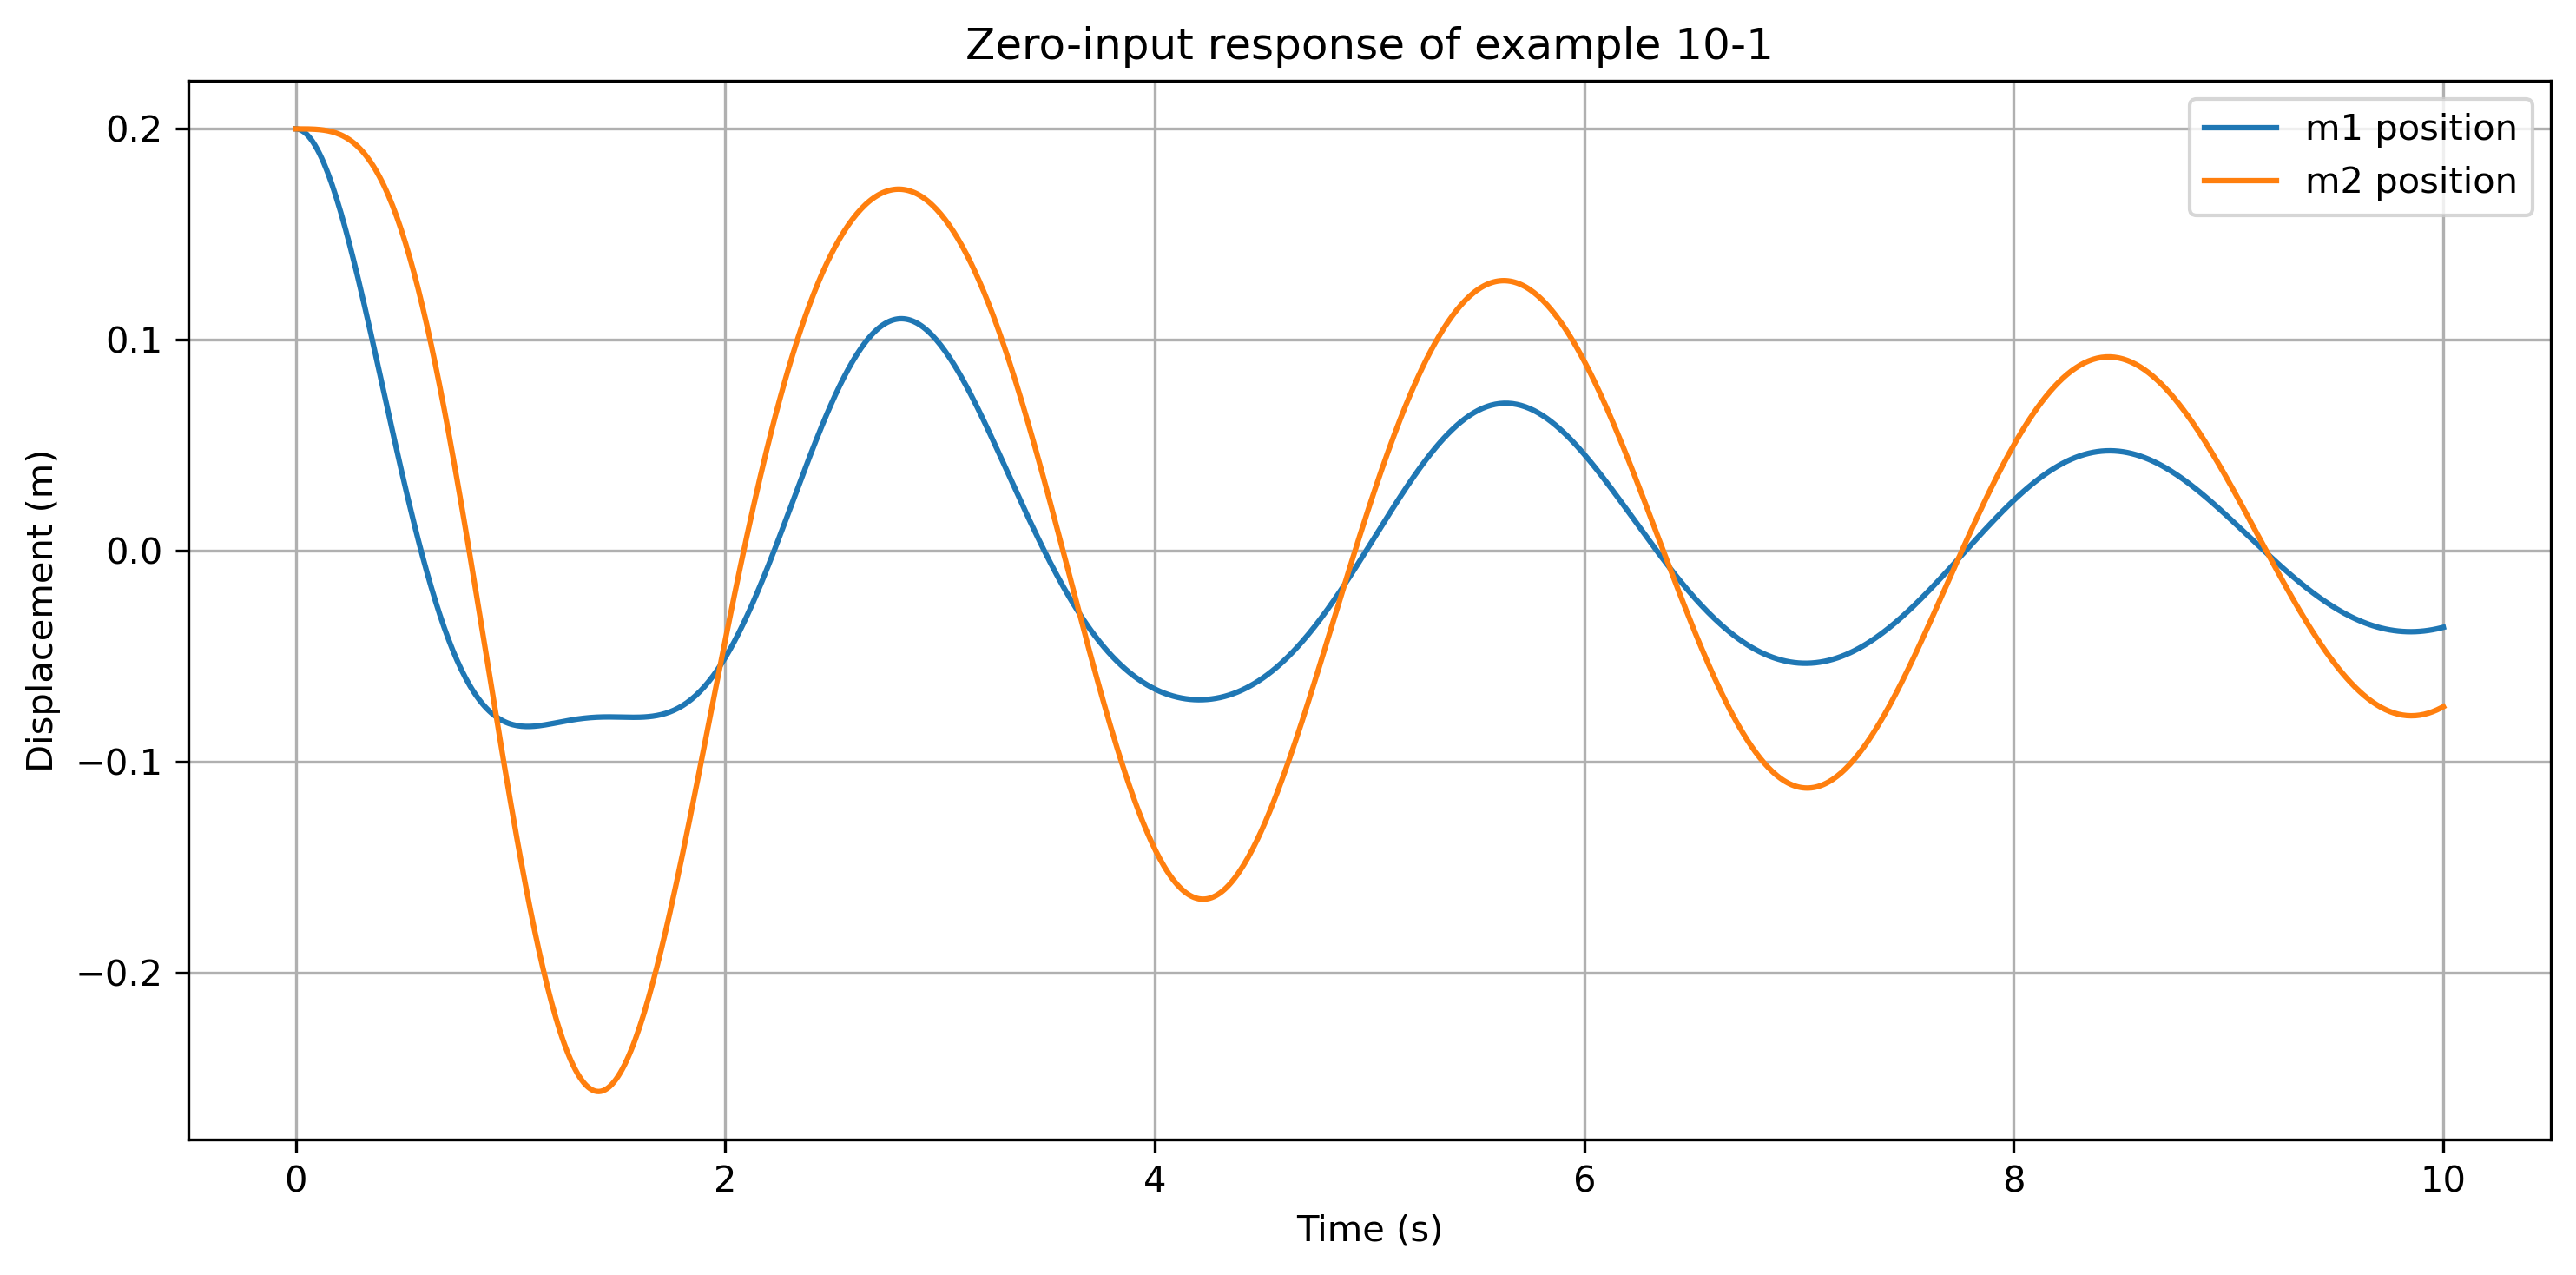
\includegraphics[width=0.8\linewidth]{images/example_10_1.png}
	\caption{Open-loop output response.}
	\label{fig:10_1}
\end{figure}

\end{example}

\subsection{Systems Modeled by Constant Coefficient Linear Difference Equations}

An $n$-th order (linear constant-coefficient) difference equation is given by
\begin{equation}
	\sum_{i=0}^n{a_iy(k+i)}=\sum_{i=0}^m{b_iu(k+i)}
\end{equation}
Define a shift operator by the equation
\begin{equation}
	Z[y(k)]\equiv{y(k+1)}
\end{equation}
The $n$-th order linear constant-coefficient difference equation
\begin{equation}
	y(k+n)+\sum_{i=0}^{n-1}{a_iy(k+i)}=u(k)
\end{equation}
can be written as
\begin{equation}
	(Z^n+\sum_{i=0}^{n-1}{a_iZ^i})[y(k)]=u(k)
\end{equation}
The characteristic equation of this difference equation is
\begin{equation}
	Z^n+\sum_{i=0}^{n-1}{a_iZ^i}=0
\end{equation}

\section{Signal Flow Graphs}

\section{Stability, Sensitivity and Error}

\subsection{Stability}

\begin{definition} A continuous system \emph{stable} if its impulse response $y_\delta(t)$ approaches zero as time approaches infinity. Similarly, a discrete-time system is stable if its Kronecker delta response $y_\delta(k)$ approaches zero as time approaches infinity.\end{definition}

A continuous or discrete-time system can also be defined as stable if every bounded input results in a bounded output.

\subsection{Sensitivity}

Sensitivity can be given for either the transfer or the frequency response function. The sensitivity of a system to its parameters is a measure of how much either of these system functions differ from its nominal when each of its parameters differs from its nominal value. Sensitivity can also be given for systems expressed in the time domain.

For a mathematical model $T(k)$ with $k$ regarded as the only parameter, the sensitivity of $T(k)$ with respect to the parameter $k$ is defined by
\begin{equation}
	S_k^{T(k)}\equiv\frac{d\,\ln{T(k)}}{d\,\ln{k}}=\frac{dT(k)}{dk}\frac{k}{T(k)}
\end{equation}

\subsection{Error}

For the canonical feedback system, the open-loop transfer function is given by
\begin{equation}
	GH=\frac{Ks^a\prod_{i=1}^{m-a}{(s+z_i)}}{s^b\prod_{i=1}^{n-b}{s+p_i}}
\end{equation}
We only consider the case where $b\geq{a}$ and $l\equiv{b-a}$.

A canonical system whose open-loop transfer function can be written in the form
\begin{equation}
	GH=\frac{K\prod_{i=1}^{m-a}{(s+z_i)}}{s^l\prod_{i=1}^{n-a-l}{s+p_i}}\equiv\frac{KB_1(s)}{s^lB_2(s)}
\end{equation}
where $l\geq{0}$ and $-z_i$ and $-p_i$ are the nonzero finite zeros and poles of $GH$, respectively, is called a type $l$ system.

Three criteria of the effectiveness (of feedback) in a stable type $l$ unity feedback system are
\begin{itemize}
	\item position (step) error constant
	\item velocity (ramp) error constant
	\item acceleration (parabolic) error constant
\end{itemize}

\subsection{Specifications}

We define an open-loop frequency response function $GH(\omega)$. For continuous systems $GH(\omega)\equiv{GH(j\omega)}$ and for discrete-time systems $GH(\omega)\equiv{GH(e^{j\omega{T}})}$. There are seven frequency-domain specifications which we will cover:
\begin{itemize}
	\item Phase crossover frequency, $\omega_\pi$
	\item Gain margin
	\item Gain crossover frequency, $\omega_\mathrm{1}$
	\item Phase margin, $\phi_\mathrm{PM}$
	\item Delay time, $T_d$
	\item Cutoff frequency, $\omega_c$ or $f_c$
	\item Bandwidth, BW
	\item Cutoff rate
	\item Resonance peak, $M_p$
	\item Resonant frequency, $\omega_p$
\end{itemize}

When using time-domain specifications, we define them in terms of responses to either unit step, ramp or parabolic inputs. We look at both steady state and transient responses. Steady state performance specifications include $K_p$, $K_v$ and $K_a$. The transient response performance specifications which we will cover are as follows:
\begin{itemize}
	\item Overshoot
	\item Delay time, $T_d$
	\item Rise time, $T_r$
	\item Settling time, $T_s$
	\item Dominant time constant, $\tau$
\end{itemize}

\section{Nyquist Analysis and Design}

\subsection{Mapping}

Let us consider a complex variable $s=\sigma+j\omega$. We will denote a complex transfer function of $s$ as $P(s)$. Let us also consider a complex variable $z=\mu+j\nu$ and denote a discrete-time (system) complex transfer function of $z$  as $P(z)$. For the first variable and transfer function we create two graphs: (1) the $s$-plane which has $j\omega$ on the ordinate and $\sigma$ on the abscissa, (2) the $P(s)$-plane which has $\mathrm{Im}\,P$ on the ordinate and $\mathrm{Re}\,P$ on the abscissa. The function $P$ maps points of the $s$-plane into the $P(s)$-plane. Similarly, $P(z)$ is a mapping or transformation from the $z$-plane to the $P(z)$-plane. For Nyquist stability plots, the locus of points in the $s$-plane which are chosen to map is called the Nyquist path. A polar plot is constructed in the $P(s)$-plane by taking $s=0+j\omega$.  

\subsection{Examples}

\begin{example}
	Consider a system with the open-loop transfer function
	\begin{equation}
		GH_1(s)=\frac{K}{s(s+p_1)(s+p_2)}\quad{K_1,p_1,p_2>0}
	\end{equation}

	We create the Nyquist (polar) plot using the following code
\begin{verbatim}
import numpy
import matplotlib.pyplot as plt
import control

K1 = 1
p1 = 0.5
p2 = 1

numerator = K1
denominator = numpy.poly([0, -p1, -p2])
GH = control.TransferFunction(numerator, denominator)

plt.figure()
control.nyquist(GH, omega_limits=(0.01, 100), omega_num=1000)
plt.show()
\end{verbatim}

\end{example}

\begin{example}
	The general transfer function of a continuous sytem lead compensator is
	\begin{equation}
		P_\mathrm{Lead}(s)=\frac{s+a}{s+b}\quad{b>a}
	\end{equation}
	This compensator has a zero at $s=-a$ and a pole at $s=-b$. The general transfer function of a continuous system lag compensator is
	\begin{equation}
		P_\mathrm{Lag}(s)=\frac{a(s+b)}{b(s+a)}\quad{b>a}
	\end{equation}
	However, in this case the zero is at $s=-b$ and the pole is at $s=-a$. The gain factor $a/b$ is included because of the way it is usually mechanized. The general transfer function of a continuous system lag-lead compensator is
	\begin{equation}
		P_\mathrm{LL}(s)=\frac{(s+a_1)(s+b_2)}{(s+b_1)(s+a_2)}\quad{b_1>a_1,b_2>a_2}
	\end{equation}
	This compensator has two zeros and two poles. For mechanization considerations, the restriction $a_1b_2=b_1a_2$ is usually imposed.
	
	Say that we have a continuous system with an open-loop frequency response function given by
	\begin{equation}
		GH(s)=\frac{K_1}{s(s+p_1)(s+p_2)}\quad{p_1,p_2,K_1>0}
	\end{equation}
	Furthermore, suppose that the system is stable and the pase margin is greater than 45 degrees. However, for a given application, the phase margin is too large, causing a longer than desire delay time in the system transient response. Also, the steady state error is too large, or, equivalently, the velocity error constant $K_v$ is too small by a factor of $\lambda>1$. The system can be modified by a combination of gain factor compensation to meet the stead state specification and phase lead compensation to improve the transient response. We first add the gain factor $\lambda$ to the system resulting the open-loop transfer function
	\begin{equation}
		GH(s)=\frac{\lambda{K_1}}{s(s+p_1)(s+p_2)}\quad{p_1,p_2,K_1>0}
	\end{equation}
	After this, we would like to add a lead network. However, the lead network would attenuate the lower frequencies. So we must increase the gain by $b/a$ while adding the lead compensator. When the gain is increased before adding the lead compensator, the system may become unstable, and the resulting open-loop transfer function is
	\begin{equation}
		GH(s)=\frac{\lambda{K_1}(b/a)}{s(s+p_1)(s+p_2)}\quad{p_1,p_2,K_1>0}
	\end{equation}
	The lead network can then be inserted in front of the gain-factor amplifier to obtain the final system response
	\begin{equation}
		GH(s)=\frac{\lambda{K_1}(b/a)(s+a)}{s(s+p_1)(s+p_2)(s+b)}\quad{p_1,p_2,K_1>0}
	\end{equation}
	
	The same procedure can be used to add lag compensation to the uncompensated system.
	
\begin{verbatim}
import numpy
import matplotlib.pyplot as plt
import control

K1 = 1
p1 = 0.5
p2 = 1

numerator = K1
denominator = numpy.poly([0, -p1, -p2])
GH = control.TransferFunction(numerator, denominator)

a = 1 # numerator = [1, a]
b = 2 # denominator = [1, b]
P = control.TransferFunction([1, a], [1, b]) # P_lead

compensated = P * GH

omega = numpy.logspace(-2, 2, 500)
GH_response = control.frequency_response(GH, omega)
compensated_response = \
	control.frequency_response(compensated, omega)

H = GH_response.fresp[0, 0, :]
Hc =  compensated_response.fresp[0, 0, :]

fig, (ax1, ax2) = plt.subplots(1, 2, figsize=(12, 6))

ax1.plot(H.real.flatten(), H.imag.flatten(),
		label='Uncompensated', color='blue')
ax1.plot(Hc.real.flatten(), Hc.imag.flatten(),
		label='Compensated', color='orange')
theta = numpy.linspace(0, 2 * numpy.pi, 500)
ax1.plot(numpy.cos(theta), numpy.sin(theta),
		'--', color='gray', label='Unit Circle')
ax1.axhline(0, color='gray', linestyle='--')
ax1.axvline(0, color='gray', linestyle='--')
ax1.set_xlim(-10, 1)
ax1.set_ylim(-10, 1)
ax1.set_title("Full Nyquist Plot")
ax1.set_xlabel("Re")
ax1.set_ylabel("Im")
ax1.legend()
ax1.grid(True)

ax2.plot(H.real.flatten(), H.imag.flatten(),
		label="Uncompensated", color='blue')
ax2.plot(Hc.real.flatten(), Hc.imag.flatten(),
		label='Compensated', color='orange')
ax2.plot(numpy.cos(theta), numpy.sin(theta),
		'--', color='gray', label='Unit Circle')
ax2.axhline(0, color='gray', linestyle='--')
ax2.axvline(0, color='gray', linestyle='--')
ax2.set_xlim(-2, 2)
ax2.set_ylim(-2, 2)
ax2.set_title('Nyquist (detail)')
ax2.set_xlabel('Re')
ax2.set_ylabel('Im')
ax2.legend()
ax2.grid(True)

plt.tight_layout()
plt.show()
\end{verbatim}

\begin{figure}[htbp]
	\centering
	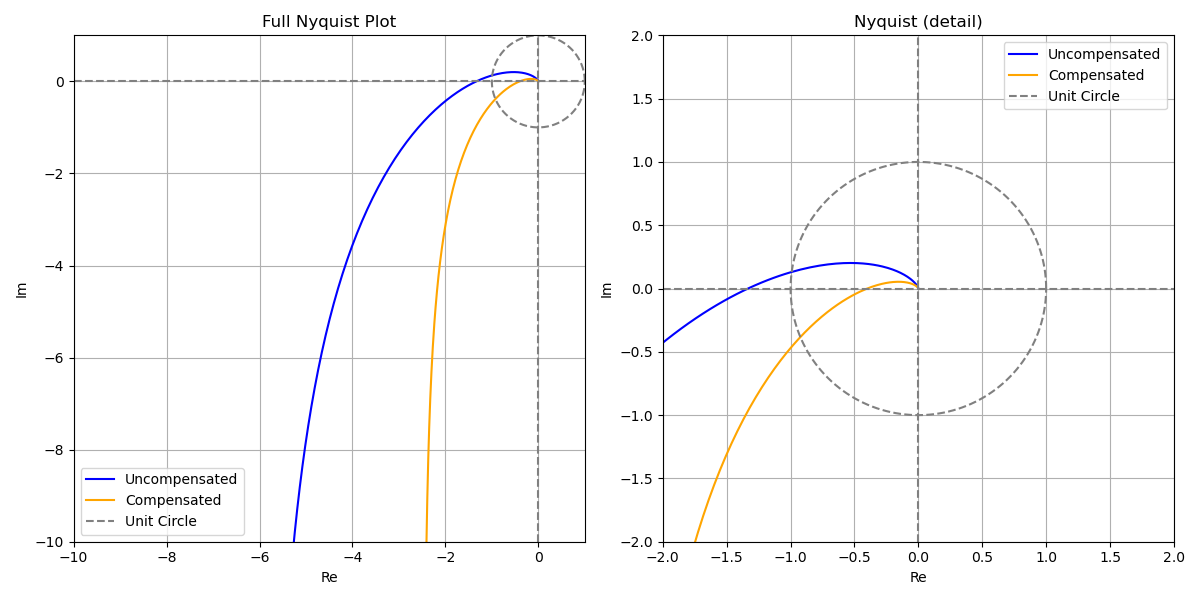
\includegraphics[width=0.7\textwidth]{images/example_11_3.png}
	\caption{Nyquist plot showing system with and without compensation from a lead compensator.}
	\label{fig:11_3}
\end{figure}

\end{example}

\begin{example}
	The general transfer function of a digital lead compensator is
	\begin{equation}
		P_\mathrm{Lead}(z)=\frac{K_\mathrm{Lead}(z-z_c)}{z-p_c}\quad{z_c>p_c}
	\end{equation}
	This compensator has a zero at $z=z_c$ and a pole at $z=p_c$. Its steady state gain is
	\begin{equation}
		P_\mathrm{Lead}(1)=\frac{K_\mathrm{Lead}(1-z_c)}{1-p_c}
	\end{equation}
	The gain factor $K_\mathrm{Lead}$ is included in the transfer function to adjust its gain at a given $\omega$ to a desired value. The general transfer fucntion of a digital lag compensator is
	\begin{equation}
		P_\mathrm{Lag}(z)=\frac{(1-p_c)(z-z_c)}{(1-z_c)(z-p_c)}\quad{z_c<p_c}
	\end{equation}
	This compensator has a zero at $z=z_c$ and a pole at $z=p_c$. The gain factor $(1-p_c)/(1-z_c)$ is included so that the low frequency or steady state gain $P_\mathrm{Lag}(1)=1$, analogous to the continuous-time lag compensator.

	Digital lag and lead compensators can be designed directly from $s$-domain specifications by using the transform between the $s$-domain and the $z$-domain defined by $z=e^{sT}$.
\end{example}


\begin{example}
	A proportional (P) controller has an output $u$ proportional to its input $e$, that is, $u=K_pe$, where $K_p$ is the proportionality constant. A derivative (D) controller has an output proportional to the derivative of its input $e$, that is, $u=K_Dde/dt$, where $K_D$ is a proportionality constant. An integral (I) controller has an output $u$ proportional to the integral of its input $e$, that is, $u=K_I\int{e(t)\,dt}$, where $K_I$ is a proportionality constant.  PD, PI, DI, and PID controllers are combinations of proportional (P), derivate (D), and integral (I) controllers. For example, the output $u$ of a PD controller has the form
	\begin{equation}
		u_{PD}=K_Pe+K_D\frac{de}{dt}
	\end{equation}
and the output of a PID controller has the form
	\begin{equation}
		u_{PD}=K_Pe+K_D\frac{de}{dt}+K_I\int{e(t)\,dt}
	\end{equation}
	The transfer function of this PID controller is
	\begin{equation}
		P_\mathrm{PID}(s)\equiv\frac{U_\mathrm{PID}(s)}{E(s)}=K_P+K_Ds+\frac{K_I}{s}=\frac{K_Ds^2+K_Ps+K_I}{s}
	\end{equation}
	This controller has two zeros and one pole. It is similar to the lag-lead compensator of the previous example except that the smallest pole is at the origin (an integrator) and it does nto have the second pole. It is typically mechanized in an analog or digital computer. 
\end{example}

\section{Root Locus Analysis and Design}

\section{Bode Analysis and Design}

\section{Miscellaneous Topics}

\subsection{Non-linear Control Systems}

\subsection{Controllability and Observability}

\subsection{State Feedback}

\subsection{Random Inputs}

\subsection{Optimal Control Systems}

\subsection{Adaptive Control Systems}

\chapter{Signal Processing}

This chapter represents a brief review of signal processing before continuing into image processing. The content of this chapter may be entirely omitted from any review or robotics course.

\section{IIR Digital Filter Design}

An infinite impulse response (IIR) filter is characterized by an impulse response of infinite duration.

\subsection{Bilinear Transformation}

One IIR digital filter (DF) design method is the bilinear transformation (BT) of classic analog filters. BT uniquely aps the entire left half of the $s$-plane into the interior of the unit circle in the $z$-plane. The design procedure is as follows:
\begin{enumerate}
	\item Design formulas -- generate analog poles and zeros of Butterworth, Chebyshev, and elliptic lowpass filters
	\item Frequency band transformation formulas -- converts analog lowpass filters into analog highpass, bandpass, and bandstop filters
	\item Bilinear transformation -- maps poles in the $s$-plane to poles in the $z$-plane
\end{enumerate}

For the linear network to be causal and stable (1) the transfer function should be a rational function of $s$ with real coefficients, (2) the poles of the analog filter must lie in the left half of the $s$-plane, and (3) the degree of the numerator (polynomial) must be less than or equal to the degree of the denominator (polynomial).

\subsection{Pole-Zero Placement}

This design method involves direct placement of the poles and zeros in the $z$-plane to meet an arbitrary frequency repsonse specification.

\subsection{Complex Coefficients}

\subsection{CAD}

This is a practical method for designing IIR digital filters with aribitrary, prescribed magnitude characteristics.

\section{FIR Digital Filter Design}

A finite impule response (FIR) filter is characterized by an impulse response of finite duration.

\section{Fourier Transform Algorithms}

\section{Random Processes, Power Spectra and Noise}

\subsection{Random Processes}

In this section we look at the effect of a random process (RP) on a a system. A wide-sense stationary (WSS) process only requires that the first and second moments are not function of time, and that the autocorrelation function depends only on the time difference. An ergodic random process requires that any statistic calculated by averaging over all members of an ergodic ensemble at a a fixed time can be calculated by averaging over all time on a single representative member of the ensemble; that is, time averages equal ensemble averages.

Let the autocorrelation functions (ACF) of the input and output processes be given by $\phi_{xx}(m)$ and $\phi_{yy}(m)$, or
\begin{align}
	\phi_{xx}(m)&=E[x(n)x(n+m)]=\lim_{x\to\infty}{\frac{1}{2N+1}\sum_{n=-N}^N{x(n)x(n+m)}}\\
	\phi_{yy}(m)&=E[y(n)y(n+m)]=\lim_{x\to\infty}{\frac{1}{2N+1}\sum_{n=-N}^N{y(n)y(n+m)}}
\end{align}
If the process is assumed to be WSS, the ACF depends only on the time difference; in that case, the system output process ACF is given by
\begin{equation}
	\phi_{yy}(m)=\sum_{i=-\infty}^\infty\sum_{j=-\infty}^\infty{h(i)h(i+j)\phi_{xx}(m-j)}
\end{equation}
The CCF of two discrete-time random proceses $x(n)$ and $y(n)$ that are jointly WSS RPs is
\begin{equation}
	\phi_{xy}(m)=E[x(n)y(n+m)]
\end{equation}
The CCF of the input $x(n)$ and response $y(n)$ of a discrete-time linear system can then be given as
\begin{equation}
	\phi_{xy}(m)=\sum_{j=-\infty}^\infty{h(j)\phi_{xx}(m-j)}
\end{equation}
The autocovariance (ACVF) and cross-covariance (CCVF) functoins of two stationary RP $x(n)$ and $y(n)$ are given by
\begin{align}
	\gamma_{xx}(m)&=E\{[x(n)-m_x][(x(n+m)+m_x)]\}=\phi_{xx}(m)-m^2_x\\
	\gamma_{xy}(m)&=E\{[x(n)-m_x][(y(n+m)-m_y)]\}=\phi_{xy}(m)-m_xm_y
\end{align}
respectively. The Z-transform of $\gamma_{xx}(m)$ and $\gamma_{xy}(m)$ are given by $\Gamma_{xx}(z)$ and $\Gamma_{xy}(z)$, respectively. The Z-transforms exist only when $m_x=-$.

\subsection{Power Spectra}

The Z-transform and the inverse Z-transform of the ACF of a zero-mean WSS discrete-time RP $x(n)$ form a transform pair $\mathbf{\Phi}_{xx}(z)\leftrightarrow\phi_{xx}(m)$ as shown by
\begin{align}
	\mathbf{\Phi}_{xx}(z)&=\sum_{m=-\infty}^{\infty}{\phi_{xx}(m)z^{-m}}\\
	\phi_{xx}(m)&=\frac{1}{2{\pi}j}\oint_c{\mathbf{\Phi}_{xx}(z)z^{m-1}\,dz}
\end{align}
where the power spectral density (PSD) is defined as the Z-transform of the ACF with $z=e^{j2{\pi}fT}$ or
\begin{equation}
	P_{xx}(f)=\mathbf{\Phi}_{xx}(e^{j2{\pi}fT})=\sum_{m=-\infty}^{\infty}{\phi_{xx}(m)e^{j2{\pi}fT}}
\end{equation}
The Z-transform of the CCF is given by
\begin{equation}
	\mathbf{\Phi}_{xy}(z)=\sum_{m=-\infty}^{\infty}{\phi_{xy}(m)z^{-m}}
\end{equation}
The cross-power spectral density (CPSD) of two functions is the Z-transform of their CCF with $z=e^{j2{\pi}fT}$ or
\begin{equation}
	P_{xy}(f)=\mathbf{\Phi}_{xy}(e^{j2{\pi}fT})=\sum_{m=-\infty}^{\infty}{\phi_{xy}(m)e^{j2{\pi}fT}}
\end{equation}
For a linear system with response $y(n)$, input $x(n)$ and impulse response $h(n)$, we can show
\begin{align}
	\mathbf{\Phi}_{yy}(z)&=H(z)H(z^{-1})\mathbf{\Phi}_{xx}(z)\\
	P_{yy}(f)&=\mathbf{\Phi}_{yy}(e^{j2{\pi}fT})=|H(e^{j2{\pi}fT})|\mathbf{\Phi}_{xx}(e^{j2{\pi}fT})
\end{align}
This says that hte the PSD of the output process of a discrete-time linear system is equal to the PSD of the input process times the squared magnitude response of the system. We can then show that the CPSD is
\begin{align}
	\mathbf{\Phi}_{xy}(z)&=H(z)\mathbf{\Phi}_{xx}(z)\\
	P_{xy}(f)&=H(e^{j2{\pi}fT})\mathbf{\Phi}_{xx}(e^{j2{\pi}fT})=H(e^{j2{\pi}fT})P_{xx}(f)
\end{align}
Consider two linear time-invariant systems with outputs $v(nT)$ and $w(nT)$, respectively, inputs $x(nT)$ and $y(nT)$, respsectively, and impulse responses $h_1(n)$ and $h_2(n)$, respectively. The CPSD is given by
\begin{equation}
	\mathbf{\Phi}_{vw}(z)=H_1(z)H_2(z^{-1})\mathbf{\Phi}_{xy}(z)
\end{equation}

\subsection{Noise}

The ACF and PSD of white noise are expressed by
\begin{align}
	\phi_{xx}(m)&=\sigma_x^2\delta(m)\\
	P_{xx}(f)&=\mathbf{\Phi}_{xx}(e^{j2{\pi}fT})=\sigma_x^2
\end{align}
Therefore, the response of a digital fitler to a white-noise input is
\begin{equation}
	P_{yy}(f)=\sigma_x^2|H(e^{j2{\pi}fT})|^2
\end{equation}
With an input with zero mean and the variance (second moment) $\sigma_x^2$, the response of a system with an impulse response $h(n)$ is
\begin{equation}
	\sigma_y^2=\sigma_x^2\sum_{n=0}^{\infty}{h^2(n)}
\end{equation}
Suppose that we would like to determine the average output power of a filter to a white-noise random process with zero mean and variance $\sigma_x^2$. For the ACF with $m=0$, we find the avaerage power in the input is
\begin{equation}
	\phi_{xx}(0)=E[x^2(n)]=\frac{1}{2{\pi}j}\oint_c{\mathbf{\Phi}_{xx}(z)z^{m-1}\,dz}=\sigma_x^2
\end{equation}
The average output power is then given by
\begin{equation}
	\phi_{yy}(0)=\frac{1}{2{\pi}j}\oint_c{\sigma_x^2H(z^{-1})H(z)z^{-1}\,dz}
\end{equation}

\chapter{Image Processing}

Morphological (image) processing involves tools derived using mathematical set theory to extract components of the image that may describe or represent (the shape of) regions in the image. Image segmentation involves subdividing an image into its constituent regions or objects. We will not treat image segmentation in detail here. Object recognition is the recognition of objects or patterns which can be considered individual regions in an image.

\section{Image Registration}

Brown divides image registration into four classes of problems: (1) multimodal registration, (2) template matching, (3) viewpoint registration and (4) temporal registration. Multimodal registration is registration of the same scene acquired from different sensors. Template registration is finding a match for a reference pattern in an image. Viewpoint registration is registration of images taken from different viewpoints. Finally, temporal registration is registration of the same scene taken at different times or under different conditions.

Given two images $I_1(x,y)$ and $I_2(x,y)$, image registration is the mapping between the two images which can be expressed as
\begin{align}
	I_2(x,y)&=g(I_1(f(x,y)))\\
	&=g(I_1(f_x(x,y),f_y(x,y)))
\end{align}

The most commone general transformations of images are rigid, affine, projective, perspective and global polynomial. An affine transformation is a combination of scaling, translation and rotation. It can be represented by the equation
\begin{equation}
	\begin{pmatrix}
		x_2\\
		y_2
	\end{pmatrix}=
	\begin{pmatrix}
		t_x\\
		t_y
	\end{pmatrix}+
	s\begin{pmatrix}
		\cos{\theta}&-\sin{\theta}\\
		\sin{\theta}&\cos{\theta}
	\end{pmatrix}
	\begin{pmatrix}
		x_1\\
		y_1
	\end{pmatrix}
\end{equation}

\backmatter

\end{document}

